\section{Internal Background}
\label{sec:background}

A run without any radioactive source has been recorded to study the internal background of the detectors. The resulting spectrum for channel 0 is shown in fig. \ref{fig:bkg}.\\

$^{138}$La decays 66.4\% by electron capture to $^{138}$Ba, which emits a 1435.80 keV gamma-ray and the Ba X-rays. The remaining 33.6\% decays by $\beta$− emission to $^{138}$Ce, releasing a 788.74 keV gamma-ray. A bremmstrahlung continuum can be observed in the spectra extending to the beta end point at 255 keV. \\
Because the lanthanum atoms are decaying inside the detector, neither of the full-energy gamma-rays appear in the spectra as expected; both are summed – the 788.74 keV with its accompanying beta particles and the 1435.80 keV with the electron capture X-rays. At higher energies, there is evidence of low level alpha emitting contamination due to $^{227}$Ac contamination. 

\begin{figure}[h!]
\centering
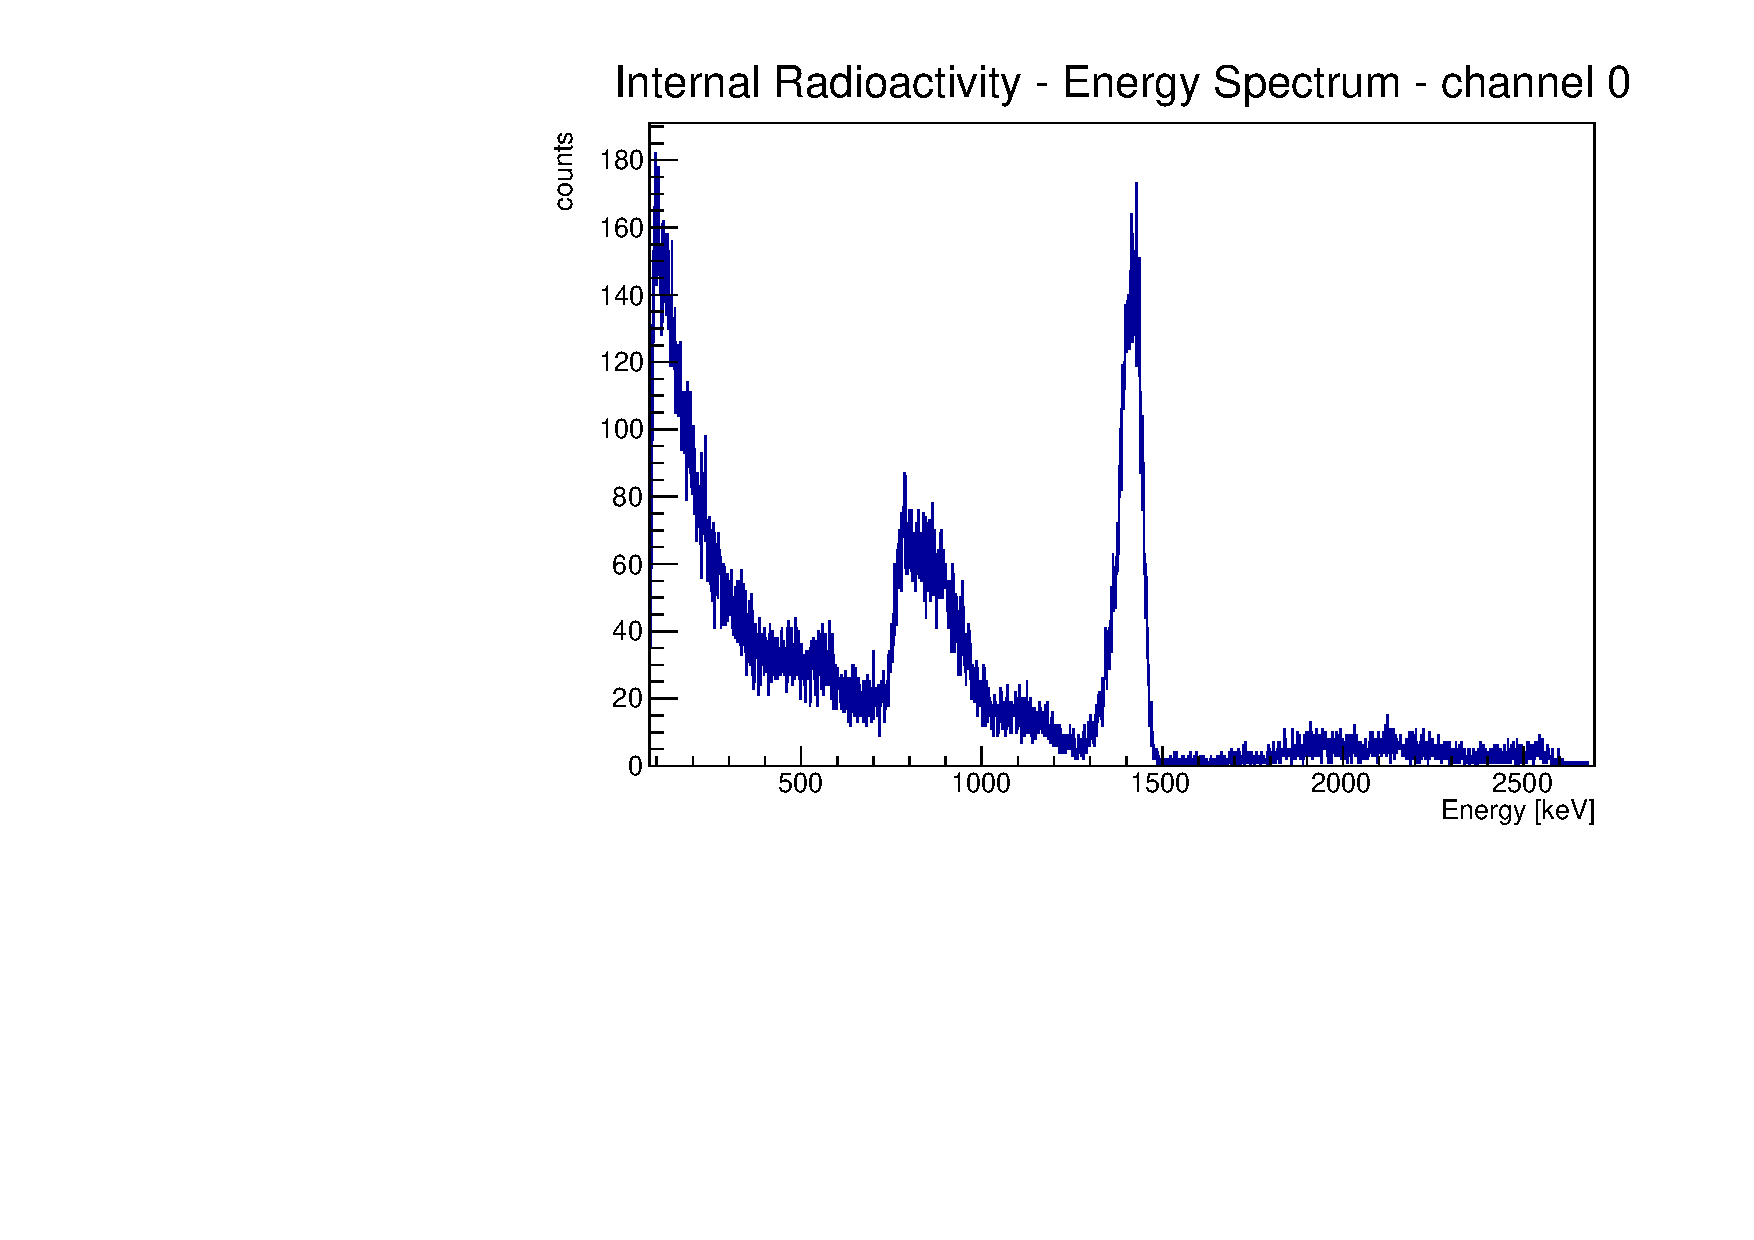
\includegraphics[width=0.6\textwidth]{Images/analysis/bkg/bg.pdf}
\caption{Background spectrum of the first detector. The three main features of the spectrum are clearly visible.}
\label{fig:bkg}
\end{figure}